%-------------------------------------------------------------------------------
% This file provides a skeleton ATLAS note.
% \pdfinclusioncopyfonts=1
% This command may be needed in order to get \ell in PDF plots to appear. Found in
% https://tex.stackexchange.com/questions/322010/pdflatex-glyph-undefined-symbols-disappear-from-included-pdf
%-------------------------------------------------------------------------------
% Specify where ATLAS LaTeX style files can be found.
\newcommand*{\ATLASLATEXPATH}{latex/}
% Use this variant if the files are in a central location, e.g. $HOME/texmf.
% \newcommand*{\ATLASLATEXPATH}{}
%-------------------------------------------------------------------------------
\documentclass[NOTE, atlasdraft=true, texlive=2016, UKenglish]{\ATLASLATEXPATH atlasdoc}
\usepackage{float}
\usepackage{euler}\usepackage{pgf}
\usepackage{subcaption}
\usepackage{natbib}
\usepackage{geometry}
\usepackage{pdflscape}
% The language of the document must be set: usually UKenglish or USenglish.
% british and american also work!
% Commonly used options:
%  atlasdraft=true|false This document is an ATLAS draft.
%  texlive=YYYY          Specify TeX Live version (2016 is default).
%  coverpage             Create ATLAS draft cover page for collaboration circulation.
%                        See atlas-draft-cover.tex for a list of variables that should be defined.
%  cernpreprint          Create front page for a CERN preprint.
%                        See atlas-preprint-cover.tex for a list of variables that should be defined.
%  NOTE                  The document is an ATLAS note (draft).
%  PAPER                 The document is an ATLAS paper (draft).
%  CONF                  The document is a CONF note (draft).
%  PUB                   The document is a PUB note (draft).
%  BOOK                  The document is of book form, like an LOI or TDR (draft)
%  txfonts=true|false    Use txfonts rather than the default newtx
%  paper=a4|letter       Set paper size to A4 (default) or letter.

%-------------------------------------------------------------------------------
% Extra packages:
\usepackage{\ATLASLATEXPATH atlaspackage}
% Commonly used options:
%  biblatex=true|false   Use biblatex (default) or bibtex for the bibliography.
%  backend=bibtex        Use the bibtex backend rather than biber.
%  subfigure|subfig|subcaption  to use one of these packages for figures in figures.
%  minimal               Minimal set of packages.
%  default               Standard set of packages.
%  full                  Full set of packages.
%-------------------------------------------------------------------------------
% Style file with biblatex options for ATLAS documents.
\usepackage{\ATLASLATEXPATH atlasbiblatex}

% Package for creating list of authors and contributors to the analysis.
\usepackage{\ATLASLATEXPATH atlascontribute}

% Useful macros
\usepackage{\ATLASLATEXPATH atlasphysics}
% See doc/atlas_physics.pdf for a list of the defined symbols.
% Default options are:
%   true:  journal, misc, particle, unit, xref
%   false: BSM, heppparticle, hepprocess, hion, jetetmiss, math, process, other, texmf
% See the package for details on the options.

% Files with references for use with biblatex.
% Note that biber gives an error if it finds empty bib files.
\addbibresource{higgsDiffNote.bib}
\addbibresource{bib/ATLAS.bib}
\addbibresource{bib/CMS.bib}
\addbibresource{bib/ConfNotes.bib}
\addbibresource{bib/PubNotes.bib}

% Paths for figures - do not forget the / at the end of the directory name.
\graphicspath{{logos/}{figures/}}

% Add you own definitions here (file wz_heavy_flavor-defs.sty).
\usepackage{higgsDiffNote-defs}

%-------------------------------------------------------------------------------
% Generic document information
%-------------------------------------------------------------------------------

% Title, abstract and document 
%-------------------------------------------------------------------------------
% This file contains the title, author and abstract.
% It also contains all relevant document numbers used for an ATLAS note.
%-------------------------------------------------------------------------------

% Title
\AtlasTitle{A Deep Learning Approach to Differential Measurements of Higgs - Top Interactions in Multilepton Final States using the ATLAS Detector at the LHC}

% Draft version:
% Should be 1.0 for the first circulation, and 2.0 for the second circulation.
% If given, adds draft version on front page, a 'DRAFT' box on top of each other page, 
% and line numbers.
% Comment or remove in final version.
\AtlasVersion{0.1}

% Abstract - % directly after { is important for correct indentation
\AtlasAbstract{%
        Several theories Beyond the Standard Model predict a modification of the momentum spectrum of the Higgs Boson, without a significantly altered rate of Higgs produced in association with top quark pairs ($t\bar{t}H$). This provides a physical observable that can be used to search for new physics based on data collected by the LHC. This thesis presents techniques and preliminary results for a differential measurement of the Higgs transverse momentum in $t\bar{t}H$ events with multiple leptons in the final state, using data collected at an energy of $\sqrt{s}$ = 13 TeV by the ATLAS detector at the LHC.

This thesis also details a measurement of WZ + heavy flavor production, a significant background to $t\bar{t}H$ that is poorly understood. This study targets events with three leptons and one or two jets in the final state, using 140 $fb^{-1}$ of  $\sqrt{s}$ = 13 TeV data. A measured cross-section of $X\pm X$ fb ($X\pm X$ fb) is observed for WZ + b (WZ + charm) with 1 associated jet and $X\pm X$ fb ($X\pm X$ fb) for WZ + b (WZ + charm) with 2 assoicated jets.

Because of the challenges inherent in reconstructing the Higgs in multilepton final states, a deep learning approach is used to predict the momentum spectrum of the Higgs for these events. The regressed Higgs $p_T$ spectrum is fit to data for events with two same-sign leptons or three leptons in the final state. The fit is used to extract normalization factors for high ($p_{T}(H) > 150$ GeV) and low ($p_{T}(H) < 150$ GeV) momentum $t\bar{t}H$ events. Preliminary results are presented for 80 $fb^{-1}$ of data, with projected results shown for 140 $fb^{-1}$.

 }

% Author - this does not work with revtex (add it after \begin{document})
\author{The ATLAS Collaboration}

% Authors and list of contributors to the analysis
% \AtlasAuthorContributor also adds the name to the author list
% Include package latex/atlascontribute to use this
% Use authblk package if there are multiple authors, which is included by latex/atlascontribute
% \usepackage{authblk}
% Use the following 3 lines to have all institutes on one line
% \makeatletter
% \renewcommand\AB@affilsepx{, \protect\Affilfont}
% \makeatother
% \renewcommand\Authands{, } % avoid ``. and'' for last author
% \renewcommand\Affilfont{\itshape\small} % affiliation formatting
% \AtlasAuthorContributor{First AtlasAuthorContributor}{a}{Author's contribution.}
% \AtlasAuthorContributor{Second AtlasAuthorContributor}{b}{Author's contribution.}
% \AtlasAuthorContributor{Third AtlasAuthorContributor}{a}{Author's contribution.}
% \AtlasContributor{Fourth AtlasContributor}{Contribution to the analysis.}
% \author[a]{First Author}
% \author[a]{Second Author}
% \author[b]{Third Author}
% \affil[a]{One Institution}
% \affil[b]{Another Institution}

% If a special author list should be indicated via a link use the following code:
% Include the two lines below if you do not use atlasstyle:
% \usepackage[marginal,hang]{footmisc}
% \setlength{\footnotemargin}{0.5em}
% Use the following lines in all cases:
% \usepackage{authblk}
% \author{The ATLAS Collaboration%
% \thanks{The full author list can be found at:\newline
%   \url{https://atlas.web.cern.ch/Atlas/PUBNOTES/ATL-PHYS-PUB-2017-007/authorlist.pdf}}
% }

% ATLAS reference code, to help ATLAS members to locate the paper
\AtlasRefCode{GROUP-2017-XX}

% ATLAS note number. Can be an COM, INT, PUB or CONF note
% \AtlasNote{ATLAS-CONF-2017-XXX}
% \AtlasNote{ATL-PHYS-PUB-2017-XXX}
% \AtlasNote{ATL-COM-PHYS-2017-XXX}

% Author and title for the PDF file
\hypersetup{pdftitle={ATLAS document},pdfauthor={The ATLAS Collaboration}}

%-------------------------------------------------------------------------------
% Content
%-------------------------------------------------------------------------------
\begin{document}

\maketitle

\tableofcontents

% List of contributors - print here or after the Bibliography.
%\PrintAtlasContribute{0.30}
\clearpage

%-------------------------------------------------------------------------------
%-------------------------------------------------------------------------------
\part{Introduction}
\label{part:intro}

%------------------------------------------------------------------------------- 

\section{Introduction}
\label{sec:intro}
Particle physics is an attempt to describe the fundamental building blocks of the universe and their interactions. The Standard Model (SM) - our best current theory of fundamental particle physics - does a remarkable job of that. All known fundamental particles and (almost) all of the forces underlying their interactions can be explained by the SM, and the predictions from this theory agree with experiment to an incredibly precise degree. This is especially true since the Higgs boson, the last piece of the SM predicted decades before, was finally discovered at the Large Hadron Collider (LHC) in 2012 \cite{HIGG-2012-27}. 

Despite the success of the SM, there remains significant work to be done. For one, the SM is incomplete: it fails to provide a description of gravity, to give an explanation for the observation of Dark Matter, or to provide a mechanism for neutrinos to gain mass. Further, a Higgs boson with a mass of around 125 GeV, as observed at the LHC, gives rise to what is known a hierarchy problem - such a low mass Higgs requires a seemingly unnatural level of ``fine tuning'' that is unexplained by the SM.

A promising avenue for addressing these problems is to study the properties of the Higgs boson and the way it interacts with other particles, in part simply because these interactions have not been measured before. Its interactions with the top quark are a particularly promising place to look. Because the Higgs field is responsible for allowing particles to acquire mass, the strength of a particle's interaction with the Higgs boson is proportional to its mass. As the most massive of the fundamental particles, the top quark has the strongest coupling to the Higgs boson, making this interaction particularly interesting to study.

These interactions can be measured by directly by studying the production of a Higgs boson in association with a pair of top quarks ($t\bar{t}H$). While studies have been done measuring the overall rate of $t\bar{t}H$ production, there are several theories of physics Beyond the Standard Model (BSM) that would affect the kinematics of $t\bar{t}H$ production without altering its overall rate. This dissertation demonstrates the feasibility of performing differential measurements of the kinematics of the Higgs boson in $t\bar{t}H$ events.

%An Effective Field Theory model can be used to model the low energy effects of high energy physics.

The proton-proton collision data collected by the ATLAS detector at the LHC from 2015-2018 provides the opportunity to make this measurement for the first time. The unprecedented energy achieved by the LHC during this period - compared to past accelerators and previous runs of the LHC itself - greatly increase the rate at which $t\bar{t}H$ events are produced, and the large amount of data collected provides the necessary statistics for a differential measurement to be performed. An exploratory study into differential measurements of the Higgs transverse momentum is presented using $t\bar{t}H$ events with multiple leptons in the final state. In addition to an explanation of the techniques used, preliminary results are shown for 79.8 $fb^{-1}$ of data from proton-proton collisions at an energy $\sqrt{s} = 13$ TeV collected by the ATLAS detector from 2015-2017. Projected results are shown for the full 139 $fb^{-1}$ of data collected from 2015-2018. 

Further, a measurement of WZ produced in association with a heavy flavor jet (including both b-jets and charm jets) is performed. This process mimics the final state of $t\bar{t}H$ multilpeton events, making it an irreducible background for that analysis and many others. However, this process is poorly understood, and difficult to simulate accurately, introducing large systematic uncertainties for analyses that include it as a background. A measurement of WZ + heavy flavor in the fully leptonic decay mode is performed in an attempt to reduce this uncertainty.

This dissertation begins with a brief explanation of the SM, its limitations, and the theoretical motivation behind this workin Part \ref{part:theory}. This is followed by a description of the LHC and the ATLAS detector in Part \ref{part:lhcAtlas}. Part \ref{part:wz} details a measurement of WZ + heavy flavor. Studies of differential measurements of $t\bar{t}H$ are then described in Part \ref{part:analysis}, and preliminary results are presented. Finally, the results of these studies are summarized in the conclusion, Part \ref{part:conclusion}.



%-------------------------------------------------------------------------------

Several theories of physics Beyond the Standard Model (BSM) predict a Higgs momentum spectrum that differs from the SM, without significantly altering the rate of $t\bar{t}H$ production. These include a CP-odd Higgs Boson, and six-dimensional operators. 

The major challenge faced by each of the various $t\bar{t}H-ML$ channels in reconstructing the Higgs Boson momentum is the presence of multiple source of $E_T^{miss}$. For both channels considered, the final state includes at least two neutrinos, one originating from the Higgs decay, another from the top quarks. This means there is inherently insufficient information to fully reconstruct the Higgs. Therefore, multiple machine learning algorithms, including both boosted decision trees (BDT) created in XGBoost \ref{xgboost} and deep neural networks (dNN) created using PyTorch are employed to first identify the decay products of the Higgs and then, based on the kinematics of those decay products, predict the transverse momentum of the Higgs.

%-------------------------------------------------------------------------------
%-------------------------------------------------------------------------------
\part{Theoretical Motivation}
\label{part:theory}

%-------------------------------------------------------------------------------

\section{The Standard Model and the Higgs Boson}
\label{sec:sm}

The Standard Model of particle physics (SM) is a Quantum Field Theory (QFT) describing the known fundamental particles and their interactions. It accounts for three of the four known fundamental force - electromagnetism, the weak nuclear force, and the strong nuclear force, but not gravity. Further, the SM describes a mechanism for combining the weak and electromagnetic forces into a singular interaction, known as the electroweak force. It is a non-Abelian gauge theory, invariant under the Lie Group $SU(3)_C\bigotimes SU(2)_L\bigotimes U(1)_Y$, where $C$ refers to color charge, $L$, the weak isospin of the particle, and $Y$, the hypercharge.

%%%%%%%%%%%%%%%%%%%%%%%%%%%%%%%%%%%%%%%%%%%%%%%%%%%%%%%%%%%%%%%
\subsection{The Forces and Particles of the Standard Model}
\label{sec:forcesParticles}

The SM particles, summarized in Figure \ref{fig:SM_summary}, can be classified into two general categories based on their spin: fermions, and bosons. 

\begin{figure}[H]
\centering
   \includegraphics[width=0.75\linewidth]{figures/theory/SM_summary.pdf}
\caption{A summary of the particles of the Standard Model, including their mass, charge and spin, with the fermions listed on the left, and the bosons on the right. \cite{oerter2006the}}
\label{fig:SM_summary}
\end{figure}

Fermions are particles with $\frac{1}{2}$-integer spin, which according to the spin-statistics theorem, causes them to comply with the Pauli-exclusion principle. They can be separated into two groups, leptons and quarks, each of which consist of three generations of particles with increasing mass.

Leptons are fermions which interact via the electroweak force, but not the strong force. The three generations of leptons consist of the electron and electron neutrino, the muon and muon neutrino, the tau and tau neutrino. The quarks, by contrast, do interact via the strong force - which is to say they have color charge - in addition to the electroweak force. The three generations include the up and down quarks, the strange and charm quarks, and the top and bottom quarks. 

Each of these generations form left-handed doublets invariant under $SU(2)$ transformations. For the leptons these doublets are:

\begin{equation}
  \label{eq:lepDoublets}
  \begin{pmatrix}
    \nu_e \\
    e^{-} \\
  \end{pmatrix}_L,\:  
  \begin{pmatrix}                                                                                                                \nu_\mu \\
    \mu^{-} \\
  \end{pmatrix}_L,\: 
  \begin{pmatrix}                                                                                                            
    \nu_\tau \\
    \tau^{-} \\
  \end{pmatrix}_L
\end{equation}

And for the quarks:

\begin{equation}        
  \label{eq:quarkDoublets}
  \begin{pmatrix}                                                                                                                               
    u \\                                                                                                                                  
    d \\                                                                                                                                  
  \end{pmatrix}_L,\:                                                                                                                           
  \begin{pmatrix}                                                                                         
    s \\                                         
    c \\                                                                                                                             
  \end{pmatrix}_L,\:                                                                                                                           
  \begin{pmatrix}     
    t \\                                                                                                                            
    b \\                                                                                                                            
  \end{pmatrix}_L                
\end{equation}

For both leptons and quarks, the heavier generations can decay into the lighter generation of particles. Hence, ordinary matter generally consists of this first generation of fermions - electrons, up quarks, and down quarks. Each of these fermions has a corresponding anti-particle, which has an equal mass as its partner but oppsite charge. The fermions acquire their mass via the Higgs Mechanism, except for the neutrinos, whose mass has been experimentally confirmed but is not accounted for in the SM. 

Bosons, by contrast, have integer spin, and are therefore unconstrained by the Pauli exclusion principle. The SM includes two kinds of bosons: Gauge bosons, which are spin-1 particles that mediate the interactions between the fermions, and a single scalar, i.e. spin-0, particle - the Higgs Boson. Of the gauge bosons, the $W^+$, $W^-$ and $Z$ bosons mediate the weak interaction, while the photon mediates the electric force, and the gluon mediates the strong force. 

%%%%%%%%%%%%%%%%%%%%%%%%%%%%%%%%%%%%%%%%%%%%%%%%%%%%%%%%%%%%%%%

\subsection{The Higgs Mechanism}
\label{sec:higgsMech}

A key feature of the SM is the gauge invariance of its Lagrangian. However, any terms added to the Lagrangian giving mass to the the gauge bosons would violate this underlying symmetry of the theory. This presents a clear problem with the theory: The experimental observation that the W and Z bosons have mass seems to contradict the gauge invariance of the SM. 

Rather than abandoning gauge invariance, an alternative way for particles to acquire mass beyond adding a simple mass term to the Lagrangian was theorized by Higgs, Englert and Brout in 1964 \cite{Higgs}. This procedure for introducing masses for the gauge bosons while preserving local gauge invariance, known as the Higgs mechanism, was incorporated into the electroweak theory by Weinberg in 1967 \cite{PhysRevLett.19.1264}.  

\subsubsection{The Higgs Field}
\label{sec:higgsField}

The Higgs mechanism introduces a complex scalar $SU(2)$ doublet, $\Phi$, with the form:

\begin{equation}
  \label{eq:phiDoublet}
  \Phi = 
  \begin{pmatrix}                                                                                                           
    \phi^+ \\                                                                                                               
    \phi^0 \\                                                                                                                            
  \end{pmatrix}_L                                                                                                                    
\end{equation}

This field introduces a scalar potential to the Lagrangian of the form:

\begin{equation}
  \label{eq:higgsV}
  V(\Phi) = \mu^2|\Phi^\dagger\Phi| + \lambda (|\Phi^\dagger \Phi|)^2
\end{equation}

Where $\mu^2$ and $\lambda$ are free parameters of the new field. This represents the most general potential allowed while preversing $SU(2)_L$ invariance and renormalizability. In the case that $\mu^2 < 0$, this potential takes the form shown in Figure \ref{fig:higgspotential}.

\begin{figure}[H]
\centering
   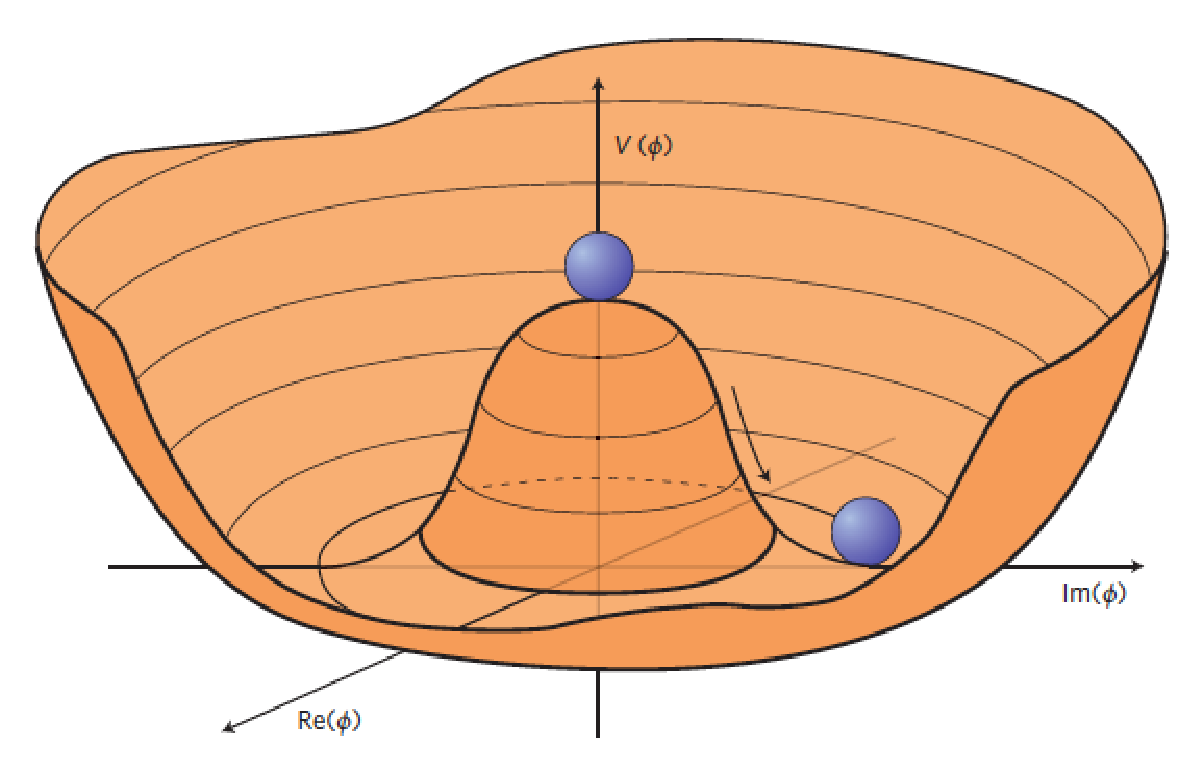
\includegraphics[width=0.75\linewidth]{figures/theory/higgspotential.eps}
\caption{The value of the Higgs potential, $V(\Phi)$ as a function of $\Phi$, for the case that $\mu^2 < 0$ \cite{Ellis:1638469}.}
\label{fig:higgspotential}
\end{figure}

The significant feature of this potential is that its minimum does not occur for a value of $\Phi = 0$. Instead, it is minimized when $|\Phi^\dagger \Phi| = -\mu^2/\lambda$. This means that in its ground state, the Higgs field takes on a non-zero value - referred to as a vacuum expectation value (VEV). So while the Higgs potential is globally symmetric, about the minimum this symmetry is broken. Since the minimum is determined only by $\Phi^\dagger \Phi$, there is some ambiguity in the particular definition of the VEV, but it is generally represented in the unitary gauge as 

\begin{equation}
  \label{eq:VEV}
  \left\langle\Phi\right\rangle = \frac{1}{\sqrt{2}}
  \begin{pmatrix}                                                                                                                               
    0 \\                                                                                                                                   
    v \\                                                                                                                                   
  \end{pmatrix}                                                                                                                       
\end{equation}

The full value of $\Phi$ can be written as 

\begin{equation}                                                                                                                                
  \label{eq:HandV}                                                                                                                                  \left\langle\Phi\right\rangle = \frac{1}{\sqrt{2}}                                                                     
  \begin{pmatrix}                                                                                                                               
    0 \\                                                                                                                   
    v + H\\                                               
  \end{pmatrix}                                                                                                                        
\end{equation}

with $v$ being the value of the VEV, and $H$ being the real value of the scalar field. 

%%%%%%%%%%%%%%%%%%%%%%%%%%%%%%%%%%%%%%%%%%%%%%%%%%%%%%%%%%%%%%%
\subsubsection{Electroweak Symmetry Breaking}
\label{sec:EWKbreaking}

The Electroweak (EWK) interaction is described in the SM by a $SU(2)_L\bigotimes U(1)_Y$ gauge theory. This theory predicts three $SU(2)_L$ gauge boson, $W^1_\mu$, $W^2_\mu$, $W^3_\mu$, and a single $U(1)_Y$ gauge boson, $B_\mu$. The couplings of these bosons to the Higgs field show up in the kinetic terms of the scalar field $\Phi$ in the Lagrangian:

\begin{equation}
  \label{eq:Lphi}
  (D_\mu\Phi)^\dagger(D^\mu\Phi) = |(\partial_\mu - \frac{ig}{2}W^a_\mu\sigma^a - \frac{ig'}{2}B_\mu Y)\phi|^2
\end{equation}

Here $D_\mu$ represents the covariant derivative required to preserve gauge invariance, $g$ and $g'$ represent coupling constant of the gauge bosons, $\sigma^a$ denotes the Pauli matrices of $SU(2)$, and $Y$ represents the hypercharge of $U(1)$. The terms in this interaction which contribute to the masses of the gauge bosons can be written as:

\begin{equation}
  \label{eq:LVEV}
  \frac{1}{2}(0,v)(\frac{g}{2}W^a_\mu\sigma^a - \frac{g'}{2}B_\mu)^2
  \begin{pmatrix}                                                                                                                               
    0 \\                                                                                                                                        
    v \\                                                                                                                                        
  \end{pmatrix}
\end{equation}

Expanding these terms into the mass eigenstates of the electroweak interaction yields four physical gauge bosons, two charged and two neutral, which are linear combinations of the fields $W^1_\mu$, $W^2_\mu$, $W^3_\mu$, and $B_\mu$:

\begin{equation}
\begin{gathered}
  \label{eq:EWKfields}
  W^\pm_\mu = \frac{1}{\sqrt{2}}(W^1_\mu \pm i W^2_\mu) \\
  Z^\mu = \frac{1}{\sqrt(g^2+g'^2)}(-g'B_\mu + gW^3_\mu) \\
  A^\mu = \frac{1}{\sqrt(g^2+g'^2)}(gB_\mu + g'W^3_\mu) \\
\end{gathered}
\end{equation}

And the masses of these fields are given by:

\begin{equation}
\begin{gathered}
  \label{eq:EWKmasses}
  M^2_W = \frac{1}{4}g^2v^2 \\
  M^2_Z = \frac{1}{4}(g^2+g'^2)v^2 \\
  M^2_A = 0 \\
\end{gathered}
\end{equation}

This produces exactly the particles we observe - three massive gauge bosons and a single massless photon. The massless photon represents the portion of the gauge symmetry, a single $U(1)$ of the electromagnetic force, that remains unbroken by the VEV.

Interactions with the Higgs field also lead to the generation of the fermion masses, which in the Lagrangian take the form:

\begin{equation}
  \label{eq:Lfermion}
  y_f (\bar{\psi}_{f,L}\phi \psi_{f,R} + \bar{\psi}_{f,R} \phi^\dagger \psi_{f,L})
\end{equation}

Here $f$ corresponds to each of the fermion flavor, and $y_f$ are matrices containing the Yukawa couplings between the Higgs field and the fermions. After symmetry breaking has occured and $\phi$ has taken on the value of the VEV as written in equation \ref{eq:VEV}, the mass terms of the fermions become $\lambda_\psi v$. Written this way, the fermion masses are proportional to their Yukawa couplings to the VEV, with masses 

\begin{equation}
\label{eq:fMass}
  m_f = y_f\frac{v}{\sqrt{2}}
\end{equation}

Based on the equation \ref{eq:HandV}, an additional mass term arises from the potential $V(\Phi)$. This term can be understood as an excitation of the Higgs field, a scalar boson with mass $m_H = 2\lambda v^2$. This is the Higgs boson, which comes about as a natural prediction of electroweak symmetry breaking. 

The fermions' Yakawa couplings to the VEV take the same form as the fermionss coupling to the Higgs boson. Therefore, the strength of a fermion's interaction with the Higgs is directly proportional to its mass. We now have a model that predicts a Higgs boson with mass $m^2_H = 2\lambda v^2$, which interacts with the fermions with coupling strength $y_f$. Because $\lambda$ and $y_f$ are free parameters of the theory, the mass of the Higgs boson and its interactions with the fermions must be measured experimentally. 

%%%%%%%%%%%%%%%%%%%%%%%%%%%%%%%%%%%%%%%%%%%%%%%%%%%%%%%%%%%%%%%

\subsection{WZ + Heavy Flavor Production}
\label{sec:WZ_theory}

Part \ref{part:wz} is dedicated to a measurement of WZ produced in association with a heavy flavor jet - namely, a charm or b-jet - in the fully leptonic channel. In the instance that both the W and Z bosons decay leptonically, this process produces a final state similar to $t\bar{t}H$, as discussed in section \ref{sec:ttH_theory}, making it an irreducible background for that analysis, and any analysis that includes multiple leptons and b-tagged jets in the final state more broadly.

\begin{figure}[H]
  \centering
  \includegraphics[width=0.35\linewidth]{figures/wz_3l.png}%                                                                 
  \includegraphics[width=0.35\linewidth]{figures/wz_3l_c.png}%                                                               
  \includegraphics[width=0.29\linewidth]{figures/wz_bbar.JPG}
  \caption{Example Feynman diagrams of WZ + heavy flavor production}
  \label{fig:wz_feynman}
\end{figure}

The b-jets produced in this process can be thought of in two different ways: either as originating from the quark ``sea'' of the initial state hadrons, or as the result of a gluon from one the colliding protons splitting into $b\bar{b}$ pairs. However, the heavy flavor contribution to the parton distribution function (PDF) of the proton is uncertain, and simulations of this process disagree depending on which of these two approaches one considers. Regardless of the modelling approach taken, the gluon splitting involved involved in producing the b-quark involves complex QCD calculations that introduce large uncertainties. The same can be said - though to a lesser degree - for charm. This makes WZ + heavy flavor difficult to accurately simulate, and introduces a large uncertainty for any analysis which includes it as a background, motivating a measurement of this process.

This measurement uses 139 $fb^{-1}$ of data collected at a center-of-mass energy of 13 TeV to verify the prediction made the Sherpa Monte Carlo generator \cite{sherpa} in simulating WZ + heavy flavor production.

%%%%%%%%%%%%%%%%%%%%%%%%%%%%%%%%%%%%%%%%%%%%%%%%%%%%%%%%%%%%%%%

\subsection{$t\bar{t}H$ Production}
\label{sec:ttH_theory}

While the SM has been tested to great precision, particularly at the LHC, it is generally accepted that it is only valid up to a certain energy scale. It is assumed that above a certain energy, at the scale where something like a Grand Unified Theory (GUT) or quantum gravity become relevant, the SM will not be applicable. Further, there are several experimental observations that the SM fails to explain. For example, the SM predicts neutrinos to be massless, despite experimental observation to the contrary, and fails to explain the observation of dark matter and dark energy.

Another example, revelant to the Higgs sector, is known as the hierarchy problem: large quantum corrections to the Higgs mass from loop diagrams, such as those shown in Figure \ref{fig:hierarchyDiagram}, are many orders of magnitude larger than the Higgs mass itself. The observed value of the Higgs mass therefore requires extremely precise cancellation between these corrections and the bare mass of the Higgs, a cancellation which seems unnatural and suggests something missing in our theoretical picture.

\begin{figure}[H]
\centering
   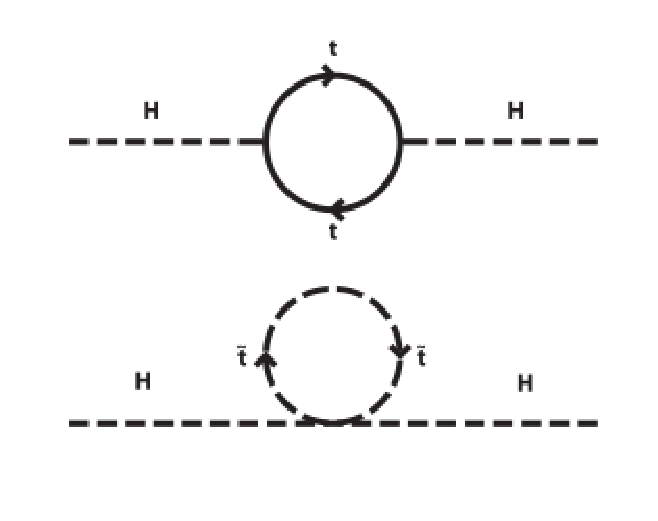
\includegraphics[width=0.5\linewidth]{figures/theory/hierarchyDiagram.eps}
\caption{Above diagram is the leading order correction to the Higgs mass via a top quark loop. Below is a stop squark loop, coming from a supersymmetric extension of the SM which, while not the focus of this paper, is an example of a process that could provide cancellation of the top diagram.}
\label{fig:hierarchyDiagram}
\end{figure}

The strength of a fermion's interaction with the Higgs, given by its Yakawa coupling, is proportionate to its mass. The top quark - as the heaviest known particle - has the strongest interaction, making this interaction particularly interesting to study. While several processes involve interactions between the Higgs and the top, some Higgs production modes include the top interaction only as a part of a loop diagram, such as the gluon-gluon fusion diagram shown in Figure \ref{fig:Hgg}. This process therefore only allows for an indirect probe of the Higgs-top Yakawa coupling, as the flavor of the quark in this diagram is not unique, and can contain other particles.

\begin{figure}[H]
\centering                                                                                                                
   \includegraphics[width=0.5\linewidth]{figures/theory/Hgg.JPG}
\caption{Diagram of a Higgs boson produced via gluon-gluon fusion.}
\label{fig:Hgg}
\end{figure}

Studying the Higgs produced in association with top quark pairs, $t\bar{t}H$, allows this interaction to be measured directly. This process, as shown in Figure \ref{fig:ttH_diagram}, involves a direct coupling between the Higgs and the top, which can be identified by the top quark pair in the final state.

\begin{figure}[H]
\centering
   \includegraphics[width=0.6\linewidth]{figures/theory/ttH_diagram.JPG}
\caption{Diagram of a Higgs boson produced in association with a pair of top quarks.}                         
\label{fig:ttH_diagram}                                                                                    
\end{figure}

The Higgs boson, as well as the top quarks, have very short lifetimes - on the order of $10^{-22}$ s and $10^{-25}$ s respectively - meaning they can only be observed via their decay products. Measuring this process is therefore a matter of identifying events with final states consistent with $t\bar{t}H$ production. 

Studies of $t\bar{t}H$ production have been reported by the ATLAS collaboration for $H\rightarrow b\bar{b}$, $H\rightarrow \gamma\gamma$ and multilepton (encompassing $H\rightarrow W^+W^-$, $H\rightarrow ZZ$ and $H\rightarrow \tau^-\tau^+$, with $H\rightarrow ZZ\rightarrow 4l$ as a separate analysis) decay modes. In multilepton final states, at least one of the light leptons, meaning either muons or electrons, originate from the Higgs decay, with other leptons originating from the decay of the top quarks. The channels targeted by this analysis - with 2 same-sign or three leptons in the final state - both involve the Higgs decaying to intermediate W bosons, $H\rightarrow W^+W^-$. The W bosons can decay either to a single lepton and a neutrino, $W\rightarrow l\nu$, providing the source for light leptons, or hadronically into two quarks. The top quarks effectively always decay to a W boson and a b-quark. The W bosons from the top quark decays provide an additional source for final state leptons in $t\bar{t}H$ events.

While the branching ratio of $H\rightarrow W^+W^-$ is smaller than $H \rightarrow b \bar{b}$ (see Table \ref{tab:H_BR}), it produces a clearer signal, as $H \rightarrow b \bar{b}$ suffers from large $t\bar{t}$ backgrounds. On the other hand, $H\rightarrow \gamma\gamma$ produces the most easily identifiable signal, but has a much smaller branching ratio than $H\rightarrow W^+W^-$. Therefore, compared with other final states of $t\bar{t}H$, the $t\bar{t}H-ML$ channel is an attractive candidate for study, as it involves a good balance between statistical power and identifiability. 

\begin{table}[H]
\centering
\begin{tabular}{lc}
\hline\hline
Decay Mode & Branching Ratio (\%) \\
\hline
$H \rightarrow b \bar{b}$ & 58.2 \\
$H\rightarrow WW^*$ & 21.4 \\
$H\rightarrow gg$ & 8.19 \\
$H\rightarrow \tau\tau$ & 6.27 \\
$H\rightarrow c\bar{c}$ & 2.89 \\
$H\rightarrow ZZ^*$ & 2.62 \\
$H\rightarrow \gamma\gamma$ & 0.227 \\
\hline
\end{tabular}
\label{tab:H_BR}
\caption{Summary of the predominant SM Higgs ($m_H = 125$ GeV) branching ratios. Particles with a star imply off-shell decays.}
\end{table} 

Searches for $t\bar{t}H$ production typically target a measurement of the signal strength parameter, $\mu_{t\bar{t}H}$, which measures the ratio of the observed cross-section and the expected cross-section according to the SM.

\begin{equation}
        \mu_{t\bar{t}H} = \frac{\sigma^{obs.}_{t\bar{t}H}}{\sigma^{SM}_{t\bar{t}H}}
\end{equation}

$t\bar{t}H$ production was observed by ATLAS using up to 79.8 $fb^{-1}$ of data collected at $\sqrt{s}$ = 13 TeV, based on a combination of five Higgs decay modes: $b\bar{b}$, $WW^*$, $\tau^{-}\tau^{+}$, $\gamma\gamma$, and $ZZ^*$ \cite{Higgs_combo}. A significance of $5.8\sigma$ was observed, compared to a $4.9\sigma$ expected significance. Since then, two analyses have published updated results ($H\rightarrow \gamma\gamma$ and $H\rightarrow ZZ^*\rightarrow 4l$) with the full Run 2 dataset, representing 139 $fb^{-1}$. Studies are still ongoing in the remaining channels.

The CMS collaboration has performed similar searched for $t\bar{t}H$, acheiving an observed (expected) significance of 5.2$\sigma$ (4.2$\sigma$) across each of the Higgs decay modes using data collected from 2011-2017 with center of mass energies of 7, 8, and 13 TeV \cite{PhysRevLett.120.231801}. 

%%%%%%%%%%%%%%%%%%%%%%%%%%%%%%%%%%%%%%%%%%%%%%%%%%%%%%%%%%%%%%%

\subsection{Differential Measurements of $t\bar{t}H$}
\label{sec:bsm}

While $t\bar{t}H$ has been observed by both the ATLAS \cite{ttH_paper} and CMS \cite{Sirunyan_2018} collaborations, these analyses have focused on measuring the overall rate of $t\bar{t}H$ production. There are several theories of physics Beyond the Standard Model (BSM), however, that could affect the kinematics of $t\bar{t}H$ production without significantly altering its overall rate \cite{Dumont_2013}.

An Effective Field Theory approach can be used to model the low energy effects of new, high energy physics, by paramaterizing BSM effects as higher dimensional operators. These additional operators can then be added to the SM Lagrangian to write an effective Lagrangian that accounts for the effects of these higher energy physics. The lowest order of these that could contribute to Higgs-top coupings are dimension-six, as represented in Equation \ref{eq:dim6}.

\begin{equation}
\label{eq:dim6}
\mathcal{L}_{eff} = \mathcal{L}_{SM} + \frac{f}{\Lambda}\mathcal{O}^6
\end{equation}

Here $\Lambda$ represents the energy scale of the new physics, $f$ is a Wilson coefficient which represents the strength of the effective coupling, and $\mathcal{O}$ is the operator. An experimental observation of any non-zero value of $f$ would be a sign of BSM physics.

The addition of these operators can be shown to modify the transverse momentum ($p_T$) spectrum of the Higgs Boson in Higg-top interactions, without significantly affecting the overall rate of $t\bar{t}H$ production \cite{Banerjee_2014}. The possible impact of these higher order effects on the Higgs $p_T$ spectrum are shown in Figure \ref{fig:eft_pt}. Here the additional operators include an effective quartic coupling between the gluon, Higgs, and a pair of top quarks, the strength of which is represented by $C_{ght}$, and a loop-induced interaction between the gluon and Higgs, $C_{GH}$. In this example the parameters are chosen such that the overall rate of $t\bar{t}H$ production remains the same as the Standard Model prediction.

\begin{figure}[H]
\centering
   \includegraphics[width=0.5\linewidth]{figures/theory/higgs_pt.PNG}
\caption{The momentum spectrum of the Higgs boson produced via top-quarks with (red) and without (blue) the presence of a particular choice of dimension-six operator.  \cite{Banerjee_2014}.}
\label{fig:eft_pt}
\end{figure}

Here the additional operators include an effective quartic coupling between the gluon, Higgs, and a pair of top quarks, shown in Equation \ref{eq:gtth}, the strength of which is represented by $C_{ght}$. $C_{GH}$ is the strength of a loop-induced interaction between the gluon and Higgs \ref{eq:gh}. In this example the values of these couplings are chosen such that the overall rate of $t\bar{t}H$ production remains the same as the Standard Model prediction.

\begin{equation}
\label{eq:gtth}
(\tilde{q}\sigma^{\mu\nu}T^At)\tilde{\phi}G^A_{\mu\nu}
\end{equation}


\begin{equation}
\label{eq:gh}
(\phi^\dagger\phi)G^A_{\mu\nu}G^{A\mu\nu}
\end{equation}


This provides a clear, physics observable that could be used to search for evidence of BSM physics using data collected at the LHC. Reconstructing the momentum spectrum of the Higgs in $t\bar{t}H$ events therefore provides a means to search for new physics in the Higgs sector.

Reconstructing the Higgs is a particular challenge in the multilepton channels of $t\bar{t}H$, due to an ambiguity arising from multiple sources of missing energy. In the $H\rightarrow \gamma\gamma$ channel, the kinematics of the Higgs can be fully reconstructed from the two photons. The same is true of $H\rightarrow b\bar{b}$, though with the additional challenge of identifying which two of the four b-quarks in the final state originated from the Higgs. By contrast, the two channels ($2lSS$ and $3l$) targeted by this analysis include at least one neutrino originating from the Higgs decay. 

\begin{figure}[H]
    \centering
    \subfigure[]{\includegraphics[width=.43\linewidth]{theory/ttH-2lSS.JPG}}%                             
    \subfigure[]{\includegraphics[width=.43\linewidth]{theory/ttH-3l.JPG}}%                                
    \caption{Feynman diagrams of $t\bar{t}H$ production with (a) two same-sign leptons and (b) three leptons in the final state.}
    \label{fig:ttH-2lSS-3l}
\end{figure}

Neutrinos are not detected by ATLAS; instead, their presence is inferred from missing transverse energy in the detector, $E^T_{miss}$. The two channels targeted here include not just a neutrino from the Higgs decay, but at least one additional neutrino from the decay of the top-quarks. This makes disentangling the contribution of the Higgs decay to $E^T_{miss}$, and thereby fully reconstructing the Higgs, impossible. This challenge motivates the use of more sophisticated machine learning techniques when attempting to perform differential measurements of the Higgs $p_T$ spectrum in the multi-lepton channels of $t\bar{t}H$. 

Chapter \ref{part:analysis} provides exploratory studies on the feasibility of differential measurements of $t\bar{t}H-ML$, specifically targeting events with two same-sign leptons ($2lSS$) or three leptons ($3l$) in the final state. This includes $H \rightarrow W^+W^-$ events, where at least one of the W bosons decays leptonically. The techniques used to reconstruct the Higgs transverse momentum spectrum are explained, and preliminary results are shown for data collected by ATLAS from 2015-2017, with projected results shown for the full 2015-2018 dataset.

%%%%%%%%%%%%%%%%%%%%%%%%%%%%%%%%%%%%%%%%%%%%%%%%%%%%%%%%%%%%%%% 



%------------------------------------------------------------------------------

\section{Limitations of the Standard Model}
\label{sec:smProblems}
While the SM has great predictive power, there are still several experimental observation that the SM fails to explain. For example, 

%------------------------------------------------------------------------------

\section{$t\bar{t}H$ Production}
\label{sec:tth_theory}
While the Higgs Boson has been discovered, its interactions with other particles have not yet been measured. Of particular interest are the interactions of the Higgs with the top quark. As the heaviest SM particle, the top quark has the strongest Yukawa coupling to the Higgs. 

By measuring the production of the Higgs boson in association with top quark pairs ($t\bar{t}H$), the higgs-top Yukawa coupling can be measured directly. 

\subsection{Higgs Production Modes}
\label{sec:higgsModes}


%------------------------------------------------------------------------------

\section{Dimension-six Operators}
\label{sec:smProblems}
Higher dimension operators are a common way to paramaterize the effects of physics at very high energies into

%------------------------------------------------------------------------------

%-------------------------------------------------------------------------------
%-------------------------------------------------------------------------------

\part{The LHC and the ATLAS Detector}
\label{part:lhcAtlas}

%-------------------------------------------------------------------------------

\section{The LHC}
\label{sec:lhc}
The Large Hadron Collider (LHC) is a particle accelerator consisting of a 17 km ring, designed to collide protons at high energy.

%------------------------------------------------------------------------------

\section{The ATLAS Detector}
\label{sec:atlas}
ATLAS (a not terribly natural acronym for ``A Toroidal LHC Apparatus'') is a general purpose detector designed to maximize the detection efficiency of all physics objects, including leptons, jets, and photons. 

%-------------------------------------------------------------------------------
%-------------------------------------------------------------------------------

\part{Search for Dimension-Six Operators}
\label{sec:evt_selection}

%-------------------------------------------------------------------------------

\section{Data and Monte Carlo Samples}
\label{sec:dataMC}
This study used data collected by the ATLAS detector over the period from 2015-2018, representing 138.9 $fb^{-1}$ of data at an energy of 13 TeV. 

Several Monte Carlo generators were used to simulate both signal and background processes. For all of these, the effects of the ATLAS detector are simulated in Geant4. 

%-------------------------------------------------------------------------------   

\section{Object Reconstruction}
\label{sec:objReco}

All analysis channels considered in this note share a common object selection for leptons and jets, as well as a shared trigger selection. 

\subsection{Trigger Requirements}

Events are required to be selected by dilepton triggers, as summarized in table \ref{tbl:trigger}.

\begin{table}[h!]
 \begin{center}
   \begin{tabular}{cc}
     \toprule
                  & Dilepton triggers (2015) \\
     \midrule
      $\mu\mu$ (asymm.)          & \verb!HLT_mu18_mu8noL1! \\
      $ee$ (symm.)               & \verb!HLT_2e12_lhloose_L12EM10VH! \\
      $e\mu,\mu e$ ($\sim$symm.) & \verb!HLT_e17_lhloose_mu14! \\
     \bottomrule
                       & Dilepton triggers (2016) \\
     \midrule
      $\mu\mu$ (asymm.)                   & \verb!HLT_mu22_mu8noL1! \\
      $ee$ (symm.)                        & \verb!HLT_2e17_lhvloose_nod0! \\
      $e\mu,\mu e$ ($\sim$symm.)          & \verb!HLT_e17_lhloose_nod0_mu14! \\
     \bottomrule

                  & Dilepton triggers (2017) \\
     \midrule
      $\mu\mu$ (asymm.)                   & \verb!HLT_mu22_mu8noL1! \\
      $ee$ (symm.)                        & \verb!HLT_2e24_lhvloose_nod0! \\
      $e\mu,\mu e$ ($\sim$symm.)          & \verb!HLT_e17_lhloose_nod0_mu14! \\
     \bottomrule
                  & Dilepton triggers (2018) \\
     \midrule
      $\mu\mu$ (asymm.)                   & \verb!HLT_mu22_mu8noL1! \\
      $ee$ (symm.)                        & \verb!HLT_2e24_lhvloose_nod0! \\
      $e\mu,\mu e$ ($\sim$symm.)          & \verb!HLT_e17_lhloose_nod0_mu14! \\
      \bottomrule
   \end{tabular}
   \caption{\label{tbl:trigger} List of lowest $p_{T}$-threshold, un-prescaled dilepton triggers used for 2015-2018 data taking.}
 \end{center}
\end{table}

\subsection{Light Leptons}
\label{subsec:lepSelection}

Electron candidates are reconstructed from energy clusters in the electromagnetic calorimeter that are associated with charged particle tracks reconstructed in the inner detector \cite{ATLAS-CONF-2016-024}.  Electron candidates are required to have $\pt > 10$ GeV and $|\eta_\textrm{cluster}| < 2.47$. Candidates in the transition region between different electromagnetic calorimeter components, $1.37 < |\eta_\textrm{cluster}| < 1.52$, are rejected. A multivariate likelihood discriminant combining shower shape and track information is used to distinguish prompt electrons from nonprompt leptons, such as those originating from hadronic showers. 

To further reduce the non-prompt contribution, the track of each electron is required to originate from the primary vertex; requirements are imposed on the transverse impact parameter significance ($|d_0|/\sigma_{d_0}$) and the longitudinal impact parameter ($|\Delta z_0 \sin \theta_\ell|$), as shown in table \ref{tbl:tightleps}.

Muon candidates are reconstructed by combining inner detector tracks with track segments or full tracks in the muon spectrometer \cite{PERF-2014-05}. Muon candidates are required to have $\pt > 10$~GeV and $|\eta| < 2.5$. All leptons are required to be isolated, and pass a non-prompt BDT selection described in detail in \cite{ttH_paper}.

\subsection{Jets}
\label{subsec:jetSelection}

%UPDATE TO PFLOW
Jets are reconstructed from calibrated topological clusters built from energy deposits in the calorimeters \cite{ATL-PHYS-PUB-2015-015}, using the anti-$k_t$ algorithm with a radius parameter $R=0.4$.  Jets with energy contributions likely arising from noise or detector effects are removed from consideration \cite{ATLAS-CONF-2015-029}, and only jets satisfying $\pt > 25$~GeV and $|\eta| < 2.5$ are used in this analysis.  For jets with $\pt < 60$~GeV and $|\eta| < 2.4$, a jet-track association algorithm is used to confirm that the jet originates from the selected primary vertex, in order to reject jets arising from pileup collisions \cite{PERF-2014-03}. 

\subsection{Missing Transverse Energy}

Because all $t\bar{t}H-ML$ channels considered include multiple neutrinos, missing transverse energy ($E_T^{miss}$) is present in each event. The missing transverse momentum vector is defined as the inverse of the sum of the transverse momenta of all reconstructed physics objects as well as remaining unclustered energy, the latter of which is estimated from low-\pt tracks associated with the primary vertex but not assigned to a hard object \cite{ATL-PHYS-PUB-2015-027}.


%------------------------------------------------------------------------------- 

%------------------------------------------------------------------------------- 

\section{Higgs Momentum Reconstruction}
\label{sec:mva}
Reconstructing the momentum of the Higgs boson is a particular challenge for channels with leptons in the final state: Because all channels include at least two neutrinos in the final state, the Higgs can never be fully reconstructed. However, the momentum spectrum can be well predicted by a neural network when provided with the four-vectors of the Higgs Boson decay products, as shown in section \ref{sec:truthLevelReco}. With this in mind, a sophisticated approach involving several layers of MVAs is used to reconstruction the Higgs momentum. 

The first layer is a Neural Network designed to select which jets are most likely to be the b-jets that came from the top decay. The kinematics of these jets are fed into the second layer, also a BDT, which is designed to identify the decay products of the Higgs Boson itself. The kinematics of these particles are then fed into a deep neural-network, which predicts the momentum of the Higgs.

\subsection{Truth Level Reconstruction}
\label{sec:truthLevelReco}

Machine Learning algorithms are trained to identify the decay products of the Higgs Boson using MC simulations of $t\bar{t}H$ events. Reconstructed physics objects are matched to truth level particles, in order to identify the parents of these reconstructed objects. 

\subsection{b-jet Identification}
\label{sec:bjetID}

In both the 3l and 2lSS channels, one or b-tagged jet is required. Therefore, for events which have exactly one, or more than two, b-tagged jets, deciding which combination of jets correspond to the top decay

\subsection{Higgs Reconstruction}
\label{sec:higgsID}

Techniques similar to the b-jet identification algorithms are employed to select the decay products of the Higgs. 

\subsection{$p_T$ Prediction}
\label{sec:ptReco}

Once the most probable decay products have been identified, their kinematics are used to reconstruct the momentum spectrum of the Higgs Boson. 

\subsection{3l Decay Mode}
\label{sec:decay3l}

In the 3l channel, there are two possible ways for the Higgs to decay, both involving intermediate W boson pairs: Either both W bosons decay leptonically, in which case the reconstructed decay consists of two leptons (referred as the fully-leptonic 3l channel), or one W decays leptonically and the other hadronically, giving two jets and one lepton in the final state (referred to as the semi-leptonic 3l channel). In order to accurately reconstruct the Higgs, it is necessary to identify which of these decays took place for each 3l event.





The first layer is a boosted decision-tree algorithm designed to select which jets are most likely to be the b-jets that came from the top decay. These jets are reconstructed by the detector a large fraction of the time

\subsection{b-jet Identification}

\subsection{Higgs Reconstruction}

\subsection{$p_T$ Prediction}


%---------------------------------------------------------------------

\section{Signal Region Definitions}
\label{sec:signal_region}
Events are divided into two channels based on the number of leptons in the final state: one with two same-sign leptons, the other with three leptons. The $3l$ channel includes events where both leptons originated from the Higgs boson as well as events where only one of the leptons 

%------------------------------------------------------------------------------------------

\subsection{Pre-MVA Event Selection}
\label{subsec:preMVA}

A preselection is applied to define orthogonal analysis channels based on the number of leptons in each event. For the 2lSS channel, the following presection is used:

\begin{itemize}
  \item Two very tight, same-charge, light leptons with $p_T > 20$ GeV
  \item $>=$4 reconstructed jets, $>=$1 b-tagged jets
  \item No reconstructed tau candidates
\end{itemize}

\begin{figure}[h!]
    \subfigure[]{\includegraphics[width=.29\linewidth]{trexPlots/stat2l_80/Plots/lep_Pt_0.png}}%                        
    \subfigure[]{\includegraphics[width=.29\linewidth]{trexPlots/stat2l_80/Plots/lep_Pt_1.png}}%                     
    \subfigure[]{\includegraphics[width=.29\linewidth]{trexPlots/stat2l_80/Plots/Mll01}}\\
    \subfigure[]{\includegraphics[width=.29\linewidth]{trexPlots/stat2l_80/Plots/nJets.png}}%                       
    \subfigure[]{\includegraphics[width=.29\linewidth]{trexPlots/stat2l_80/Plots/nbJets.png}}%                
    \subfigure[]{\includegraphics[width=.29\linewidth]{trexPlots/stat2l_80/Plots/MET.png}}\\
    \caption{}                           
    \label{fig:presel2lSS}
\end{figure}

For the 3l channel, the following selection is applied:

\begin{itemize}
  \item Three light leptons with total charge $\pm 1$
  \item Same charge leptons are required to be very tight, with $p_T > 20$ GeV
  \item Opposite charge lepton must be loose, with $p_T > 10$ GeV
  \item $>=$2 reconstructed jets, $>=$1 b-tagged jets                                                                        
  \item No reconstructed tau candidates
  \item $|M(l^+l^-)-91.2\textrm{ GeV}| > 10$~\GeV{} for all opposite-charge, same-flavor lepton pairs
\end{itemize}

\begin{figure}[h!]
    \subfigure[]{\includegraphics[width=.29\linewidth]{trexPlots/stat3l_80/Plots/lep_Pt_0.png}}%                             
    \subfigure[]{\includegraphics[width=.29\linewidth]{trexPlots/stat3l_80/Plots/lep_Pt_1.png}}%                      
    \subfigure[]{\includegraphics[width=.29\linewidth]{trexPlots/stat3l_80/Plots/Mll01}}\\                             
    \subfigure[]{\includegraphics[width=.29\linewidth]{trexPlots/stat3l_80/Plots/nJets.png}}%                          
    \subfigure[]{\includegraphics[width=.29\linewidth]{trexPlots/stat3l_80/Plots/nbJets.png}}%                          
    \subfigure[]{\includegraphics[width=.29\linewidth]{trexPlots/stat3l_80/Plots/MET.png}}\\                         
    \caption{}
    \label{fig:presel3l}                                                                                          
\end{figure}

%------------------------------------------------------------------------------------------

\subsection{Event MVA}
\label{subsec:sigBkgMVA}

Separate multi-variate analysis techniques (MVAs) are used in order to distinguish signal events from background for each analysis channel - 2lSS, 3l semi-leptonic, and 3l fully leptonic. In particular, Neural Networks produced with Tensorflow are trained using the kinematics of signal and background events derived from Monte Carlo simulations. Further, because the background composition differs for events with a high reconstructed Higgs $p_T$ compared to events with low reconstructed Higgs $p_T$, separate MVAs are produced for high and low $p_T$ regions.

Output distributions of each MVA are shown in figure \ref{fig:sigBkgScore}. Detailed explanations of each of the models can be found in section \ref{apx:MVA}.

\begin{figure}
  \subfigure[]{\includegraphics[width=.3\linewidth]{trexPlots/xgb_higgsDiff/Plots/xgb_sigBkg_2lHigh.png}}%
  \subfigure[]{\includegraphics[width=.3\linewidth]{trexPlots/xgb_higgsDiff/Plots/xgb_sigBkg_3lSHigh.png}}%
  \subfigure[]{\includegraphics[width=.3\linewidth]{trexPlots/xgb_higgsDiff/Plots/xgb_sigBkg_3lFHigh.png}}\\
  \subfigure[]{\includegraphics[width=.3\linewidth]{trexPlots/xgb_higgsDiff/Plots/xgb_sigBkg_2lLow.png}}%
  \subfigure[]{\includegraphics[width=.3\linewidth]{trexPlots/xgb_higgsDiff/Plots/xgb_sigBkg_3lSLow.png}}%
  \subfigure[]{\includegraphics[width=.3\linewidth]{trexPlots/xgb_higgsDiff/Plots/xgb_sigBkg_3lFLow.png}}
  \label{fig:sigBkgScore}
  \caption{scores}
\end{figure}

%------------------------------------------------------------------------------------------

\subsection{Signal Region Definitions}
\label{subsec:sigRegions}

Once pre-selection has been applied, channels are further refined based on the MVAs described above. The output of the model described in section \ref{sec:decay3l} is used to separate the three channel into two - Semi-leptonic and Fully-leptonic - based on the predicted decay mode of the Higgs boson. 

For each event, depending on the channel as well as the predicted $p_T$ of the Higgs derived from the algorithm described in section \ref{sec:ptReco}, a cut on the appropriate background rejection algorithm is applied. The specific selection used, and the event yield in each channel after this selection has been applied, is summarized below.

\subsubsection{$2lSS$}

\subsubsection{$3l - Semi-leptonic$}

\subsubsection{$3l - Fully-leptonic$}


%-------------------------------------------------------------------------------

\section{Systematic Uncertainties}
\label{sec:sys}
The systematic uncertainties that are considered are summarized in Table \ref{tab:SystSummary}. These are implemented in the fit either as a normalization factors or as a shape variation or both in the signal and background estimations. The numerical impact of each of these uncertainties is outlined in section \ref{sec:results}.

\begin{table}[H]
\centering
\caption{Sources of systematic uncertainty considered in the analysis. Some of the systematic uncertainties are split into several components, as indicated by the number in the rightmost column.}
\begin{tabular}{lr}
\hline\hline
Systematic uncertainty & Components           \\
\hline
\hline
Luminosity      & 1                   \\
Pileup reweighting      & 1                   \\
\textbf {Physics Objects}       &                     \\
\ \ Electron                                    & 6                   \\
\ \ Muon        & 15                  \\
\ \ Jet energy scale and resolution     & 28                  \\
\ \ Jet vertex fraction         & 1                   \\
\ \ Jet flavor tagging          & 131                 \\
\ \ $E^{miss}_T$        & 3                   \\
\hline
Total (Experimental)        & 186                    \\
\hline
\hline
\textbf {Background Modeling}           &                     \\
\ \ Cross section                       & 24                  \\
\ \ Renormalization and factorization scales    & 10                  \\
\ \ Parton shower and hadronization model               & 2                   \\
\ \ Shower tune                         & 4                   \\
\hline
Total (Signal and background modeling)       & 40                    \\
\hline
\hline
\textbf {Background Modeling}           &                     \\
\ \ Cross section                       & 24                  \\
\ \ Renormalization and factorization scales    & 10                  \\
\ \ Parton shower and hadronization model               & 2                   \\
\ \ Shower tune                         & 4                   \\
\hline
Total (Signal and background modeling)       & 40                    \\
\hline\hline
Total (Overall)                             & 226             \\
\hline\hline
\end{tabular}
\label{tab:SystSummary}
\end{table}

The uncertainty in the combined integrated luminosity is derived from a calibration of the luminosity scale using x-y beam-separation scans performed for 13 TeV proton-proton data \cite{lumi}, \cite{LUCID2}.

The experimental uncertainties are related to the reconstruction and identification of light leptons and and b-tagging of jets, and to the reconstruction of $E^{miss}_T$. 

The sources which contribute to the uncertainty in the jet energy scale \cite{jes} are decomposed into uncorrelated components and treated as independent sources in the analysis. This method decomposes the uncertainties into 30 nuiscance parameters included in the fit. A similar method is used to account for jet energy resolution (JER) uncertainties, and 8 JER uncertainty components are uncluded as NPs in the fit.

The uncertainties in the b-tagging efficiencies measured in dedicated calibration analyses \cite{btag_cal} are also decomposed into uncorrelated components. The large number of components for b-tagging is due to the calibration of the distribution of the BDT discriminant.

As mentioned in Section \ref{sec:MCsamples}, a normalization corrections and uncertainties on the estimates of non-prompt leptons backgrounds are derived using data driven techniques, decribed in detail in \cite{ttH_paper}. These are derived from a likelihood fit over various non-prompt enriched control regions, targeting several sources of non-prompt light leptons separately: external conversion electrons, internal conversion electrons, electrons from heavy flavor decays, and muons from heavy flavor decays. %These are used to derive overall fake factors for electrons from light source (e.g. photon conversions or light hadrons), electrons from heavy flavor decays (namely, charm or bottom hadrons), and a single fake factor for muons.

The normalization factor and uncertainty applied to each source of non-prompt leptons is summarized in Table \ref{tab:fakeNF}

\begin{table}[H]
\begin{center}
\begin{tabular}{c|c}
\hline\hline
Processs &  Normalization Factor\\
\hline
$NF_e^{ExtCO}$ & 1.70 $\pm$ 0.51 \\
$NF_e^{IntCO}$ & 0.75 $\pm$ 0.26 \\
$NF_e^{HF}$ & 1.09 $\pm$ 0.32 \\
$NF_{\mu}^{HF}$ & 1.28 $\pm$ 0.17 \\
\hline
\end{tabular}
\label{tab:fakeNF}
\caption{Normalization factors - with statistical and systematic uncertainties - derived from the fit over fake control regions for each source of non-prompt leptons considered.}
\end{center}
\end{table}


In addition to those derived from the control regions, several additional uncertainties are assigned to the non-prompt lepton background. An additional 25\% uncertainty on material conversions is assigned, based on the comparison between data and MC in a region where a loose electron fails the photon conversion veto. A shape uncertainty of 15\% (6\%) is assigned to the HF non-prompt electron (muon) background based on a comparison between data and MC where the second leading electron (muon) is only required to be loose. As the contribution from light non-prompt leptons is small, about 10\% percent of the contribution from HF non-prompt leptons, it is derived from the agreement between data and simulation in a LF enriched region at low values of the non-prompt lepton BDT. The resulting uncertainty is 100\%, and is taken to be uncorrelated between internal and material conversions.

Theoretical uncertainties applied to MC predictions, including cross section, PDF, and scale uncertainties are taken from theory calculations for the predominate prompt backgrounds. Following the nominal $t\bar{t}H-ML$ analysis, a 50\% uncertainty is applied to Diboson to account for the large uncertainty in estimating VV + heavy flavor. The other ``rare'' background processes - including $tZ$, rare top processes, $ttWW$, $WtZ$, $VVV$, $tHjb$ and $WtH$ - are assigned an overall 50\% normalization uncertainty as well. The theory uncertainties applied to the MC estimates are summarized in Table \ref{tab:xsecUnc}.

\begin{table}[H]                                                                                                              {\footnotesize
\centering
../ttHDiff-PUB-Note/sections/ttH_xsecUnc.tex
\caption{Summary of theoretical uncertainties for MC predictions in the analysis.}
\label{tab:xsecUnc}}
\end{table}

Additional uncertainties to account for $t\bar{t}W$ mismodelling are also applied. These include a ``Generator'' uncertainty, based on a comparison between the nominal Sherpa 2.2.5 sample, and the formerly used aMC@NLO sample, and an ``Extra radiation'' uncertainty, which includes renormalisation and factorisation scale variations of the Sherpa 2.2.5 sample.


%-------------------------------------------------------------------------------

The systematic uncertainties that are considered are summarized in table \ref{tab:systematics}. These are implemented in the fit either as a normalization factors or as a shape variation or both in the signal and background estimations. The numerical impact of each of these uncertainties is outlined in section \ref{sec:results}.

\begin{table}[h]
\centering
\caption{Sources of systematic uncertainty considered in the analysis.
Some of the systematic uncertainties are split into several components, as indicated by the number in the rightmost column.}
\begin{tabular}{lr}
\hline\hline
Systematic uncertainty & Components  	      \\
\hline
\hline
Luminosity	& 1		      \\
Pileup reweighting 	& 1		      \\
\textbf {Physics Objects}     	&		      \\
\ \ Electron                               	& 6		      \\
\ \ Muon	& 15		      \\
\ \ Jet energy scale and resolution  	& 28                  \\
\ \ Jet vertex fraction  	& 1		      \\
\ \ Jet flavor tagging   	& 131		      \\
\ \ $E^{miss}_T$  	& 3		      \\
\hline
Total (Experimental)        & 186		     \\
\hline
\hline
\textbf {Background Modeling}          	&		      \\
\ \ Cross section                 	& 24		      \\
\ \ Renormalization and factorization scales 	& 10		      \\
\ \ Parton shower and hadronization model       	& 2		      \\
\ \ Shower tune				& 4		      \\
\hline
Total (Signal and background modeling)       & 40		     \\
\hline\hline
Total (Overall)                             & 226	      \\
\hline\hline
\end{tabular}
\label{tab:SystSummary}
\end{table}

The uncertainty in the combined 2015+2016 integrated luminosity is derived from a calibration of the luminosity scale using x-y beam-separation scans performed in August 2015 and May 2016 \cite{lumi}.

The experimental uncertainties are related to the reconstruction and identification of light leptons and
 and b-tagging of jets, and to the reconstruction of $E^{miss}_T$. The sources which contribute to the uncertainty in the jet energy scale \cite{jes} are decomposed into uncorrelated components and treated as independent sources in the analysis. 

The uncertainties in the b-tagging efficiencies measured in dedicated calibration analyses \cite{btag_cal} are also decomposed into uncorrelated components. The large number of components for b-tagging is due to the calibration of the distribution of the BDT discriminant.  

The systematic uncertainties associated with the signal and background processes are accounted for by varying the cross-section of each process within its uncertainty.

%-------------------------------------------------------------------------------
                                                                
\section{Results}
\label{sec:results}
Unblinded results are shown for the 80 $fb^{-1}$ data set, as well as MC only projections of results using the full Run-2, 140 $fb^{-1}$ dataset.

%-------------------------------------------
\subsection{Results - 80 $fb^{-1}$}
\label{sec:res80}
%-------------------------------------------

A maximum likelihood fit is performed simultaneously over the regions shown in figure \ref{fig:sigRegions80}.

\begin{figure}[h!]
    \subfigure[]{\includegraphics[width=.29\linewidth]{trexPlots/stat_80/Plots/recoHiggsPt_2lSS_postFit.png}}%   
    \subfigure[]{\includegraphics[width=.29\linewidth]{trexPlots/stat_80/Plots/recoHiggsPt_3lS_postFit.png}}%    
    \subfigure[]{\includegraphics[width=.29\linewidth]{trexPlots/stat_80/Plots/recoHiggsPt_3lF_postFit.png}}\\
    \caption{}
    \label{fig:sigRegions80}
\end{figure}

\begin{figure}[h!]
    \center
    \includegraphics[width=.9\linewidth]{trexPlots/stat_80/Plots/Summary_postFit.png}
    \caption{Post-fit summary of fit.}                                                                          
    \label{fig:Summary80}
\end{figure}

\begin{figure}[H]
    \centering
    \includegraphics[width=0.7\linewidth]{trexPlots/stat_80/PieChart_postFit.png}
    \caption{Background composition of the fit regions.}
    \label{fig:pieChart80}
\end{figure} 

%-------------------------------------------

%-------------------------------------------                                                                                 
\subsection{Projected Results - 140 $fb^{-1}$}   
\label{sec:res140}
%------------------------------------------- 

\begin{figure}[h!]
    \subfigure[]{\includegraphics[width=.29\linewidth]{trexPlots/stat_140/Plots/recoHiggsPt_2lSS_postFit.png}}%             
    \subfigure[]{\includegraphics[width=.29\linewidth]{trexPlots/stat_140/Plots/recoHiggsPt_3lS_postFit.png}}%        
    \subfigure[]{\includegraphics[width=.29\linewidth]{trexPlots/stat_140/Plots/recoHiggsPt_3lF_postFit.png}}\\
    \caption{}
    \label{fig:sigRegions140}
\end{figure}

\begin{figure}[h!]
    \center
    \includegraphics[width=.9\linewidth]{trexPlots/stat_140/Plots/Summary_postFit.png}
    \caption{Post-fit summary of fit.}
    \label{fig:Summary140}
\end{figure}

\begin{figure}[H]
    \centering                                                                                                               
    \includegraphics[width=0.7\linewidth]{trexPlots/stat_140/PieChart_postFit.png}
    \caption{Background composition of the fit regions.}
    \label{fig:pieChart140}
\end{figure}

%-------------------------------------------


%------------------------------------------------------------------------------

\part{Conclusion}
\label{part:conclusion}

As search for the effects of dimension-six operators on $t\bar{t}H$ production is performed. An effective field theory approached is used to parameratize the effects of high energy physics on the Higgs momentum spectrum. The momentum spectrum is reconstructed using various MVA techniques, and the limits on dimension-six operators are limited to X. 


%-------------------------------------------------------------------------------
% If you use biblatex and either biber or bibtex to process the bibliography
% just say \printbibliography here
\printbibliography
% If you want to use the traditional BibTeX you need to use the syntax below.
%\bibliographystyle{bib/bst/atlasBibStyleWithTitle}
%\bibliography{wz_heavy_flavor,bib,ATLAS,bib/CMS,bib/ConfNotes,bib/PubNotes}
%-------------------------------------------------------------------------------

%-------------------------------------------------------------------------------
% Print the list of contributors to the analysis
% The argument gives the fraction of the text width used for the names
%-------------------------------------------------------------------------------
\clearpage
\PrintAtlasContribute{0.30}


%-------------------------------------------------------------------------------
\clearpage
\appendix
\part*{Appendices}
\addcontentsline{toc}{part}{Appendices}
%-------------------------------------------------------------------------------

\section{}

\end{document}
